\chapter{Discussion \& Conclusions}

First, there is three points that should be remarked.
 
1) The topology and efficiency of the \gls{Lightning Network} will form as a product of profitable behavior, bottom up. It will not form from intervention, where a random mesh network is seen as preferable and the actors aim to fulfill such a model.
 
2) The behavior regarded in this thesis leads to a sufficiently robust network with short average paths. Strategies that fulfill valuable niches in the network will be profitable and the emerging real network will most likely be more efficient than any conceived model as nodes struggle in the most Darwinian sense to provide liquid paths between paying nodes.

3) The revenue distribution is exponential above the 'bankruptcy' level due to inherent properties of networks. This holds true even if all nodes utilize the same strategies and are equally funded. It has been the narrative that the market dynamics would force down the fees towards the operational costs\footnote{Including \textit{time-value-of-money} and the \textit{security-risk-premium}.} - leading to low margins for \gls{node} operators with little overall upside. This is only partially true in that routing fees will be competitive but not that it will lead to a low margin business.  

\section{Limitations with simulation}



\section{Balanced Channels}

At first sight it may seem obvious that the fee price structure is flawed as it cannot incentive, e.g give a discount, for a route in such a direction so it leaves channels in a more balanced state. A change in fee structure obviously change the validity of each strategy.

Suppose there exists a channel between Alice and Bob with 10 million satoshis in it. 
Two payments, $P_{1}$ and $P_{2}$ are routed through the channel from Bob to Alice.
Both use the same amount of liquidity, 3,500,000 satoshis each, but they start from two different initial states $B_{1}$ and $B_3$.

\begin{figure}[!htb]
	\hspace*{0.7cm} 
	\centering
	\includegraphics[width=7cm]{images/protocol_upgrade.png}
	
	\label{fig:upgrade}
	\hspace*{2mm} 	
\end{figure}

The two payments would incur the same fee, 

\[ F_{P_1 P_2} = F_B + (3,500,000 * F_R / 1,000,000) \]

but leave the channels in completely different states. $P_1$ at $B_2$ and $P_2$ at $B_4$. It is of course possible to bump the channel price after $P_1$ to
be more expensive, but suppose a third larger payment $P_3$ going from $B_1$ to $B_4$ would still run into this problem.

If a naive structure, that takes the state, is considered so as the issues of such a solution arise. 

Each satoshi in the channel could be seen as a different bracket, with a different price for each satoshi moved. The channels would then broadcast a cost function instead of the fixed fee.

\begin{figure}[!htb]
	\hspace*{-0.5cm}
	\centering
	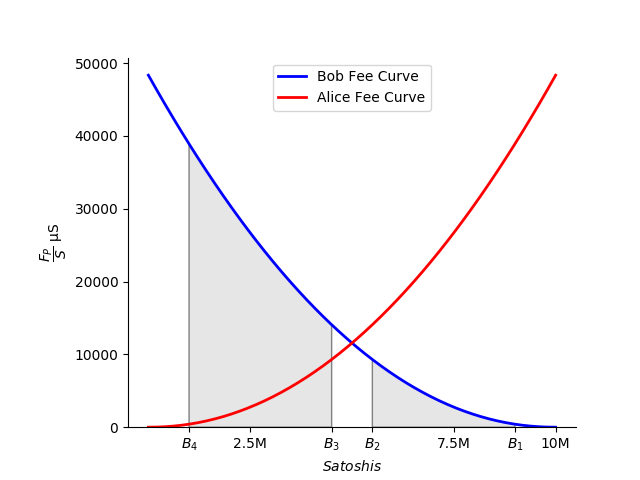
\includegraphics[width=9cm]{images/fee_scheme.png}
	\label{fig:fee scheme}
	\hspace{2mm}
\end{figure}

From the cost function the fee may be retrieved by calculating the area under the graphs. Some deterministic way to round the fee to whole satoshis and some way to verify the function is formulated correctly must be defined. 

The fees for $P_1$, $P_2$ would be very different with this brackets method.

\[ F_{P_1} = F_{B} + \int_{B_1}^{B_2} f(x) dx = F_B + 13,502,153,930 \mu S \] 

\[ F_{P_2} = F_{B} + \int_{B_3}^{B_4} f(x) dx  = F_B + 88,984,850,361 \mu S \]

Here the fees are much larger for the payment that unbalances the channel than the payment that balances it. 

However there are some clear problems with this approach. Every new payment would require each \gls{node} on the path to rebroadcast the new balance to all other nodes\footnote{As brought up by Andrea Rapitzu.~\cite{raspitzu:fee}}. Which would scale even worse than the Bitcoin bottom layer in message passing. There would also be privacy issues as any observant node could track the payments through balance updates\footnote{As brought up by ZmnSCPxj.~\cite{ZmnSCPxj:fee}}.

There is thus no clear way to 'discount' routing in a balancing direction.

It is further unclear how much immediate balance will matter for routing success and other solutions have been proposed to levitate this pressure point. E.g René Pickhardt JIT-routing~\cite{pickard:jit} and branching - utilizing multiple paths to fulfill the liquidity needed.

\section{Future work}

Future work might be interesting in many different directions.

\subsection{Protocol changes and growth}

As the lightning network protocol is still under development and small changes in the Bitcoin protocol may change the dynamics of which the nodes operate. E.g. It seem probably that funding channels by both parties will be available in the near future. \\

It is difficult to say how universal these results are although surely many strategies suggested herein will still be successful with protocol changes. Each strategy is also dependent on what every other \gls{node} in the network does. As the network grow - strategies and behavior will change. Thus the practicality of the results of these simulations are very context dependent, with introduction of new strategies, protocol changes etc. will require this model to be gradually updated to remain relevant.  

\subsection{Network theory}

Albert-László Barabási recently remarked that the bottleneck in network theory is mainly data-driven~\cite{barabasi:decade:beyond}. The \gls{Lightning Network} provides accurate network data with clear economic incentives for each actor. This may, in many ways, are unprecedented. There might be worth to study the network, in addition to its ability to scale Bitcoin, for what it suggest for networks in general. Many studies, cited herein, have been done on attachment heuristics in relation to fitness - it has however, been difficult to apply in practice to real networks. The \gls{Lightning Network} may be a better empirical test-bed for models than any preceding network. 

\subsection{Game Theory}

Much similar to Network Theory, Game theory have been difficult to use in empirical context. Especially in EGT as nature seldom have clear pay-off matrices. Even very clear examples, such as with the Bacteriophage shown by Turner and Chao~\cite{turner:chao:prisoners:dilemma, nowak:sigmund:phage}, still contains significant noise. Market data on the other hand, especially prices, is available in droves and it is arguable easier to apply game theory to economics. It usually still require effort to retrieve data, e.g. geo-locations of competing businesses. The \gls{Lightning Network} might give us further insight into regional nuances and due to completeness bridge the gap between individual strategy with full market Marshallian dynamics.    

\subsection{Fee complexity}

The optimal fee price for each edge will most likely be to expensive to calculate in the near future as the network grows. It is not uncertain how much low capacity \gls{node}s affect the network and larger operators might be able to simply prune away these nodes before calculation. Another approach is to approximate, calculating the upper and lower bounds with adjustable granularity, akin to tolerance~\cite{goldengorin:jager:tolerance}. 

\subsection{Empirical gathering}

There is still many assumptions in this the

(genetic algorithm)

(lightning factories)

